\documentclass[notes,slidesec,a4]{seminar}
\usepackage[spanish]{babel}
\usepackage[utf8]{inputenc}
\usepackage{t-gsyc-6}
\usepackage{fancybox}
\usepackage{graphics}
\usepackage{moreverb}
\usepackage{alltt}
\usepackage{html}
\usepackage{hthtml}
\usepackage{amsmath}
\usepackage[normalsize]{subfigure}
\usepackage{url}
\usepackage{listings}
\usepackage{eurosym}

\title{\color{red}{BT Studio: a ROS Behaviour-Tree web IDE}}
\author{Asociación de Robótica e Inteligencia Artificial JdeRobot}
\cop{JdeRobot}
\address{CIF G88145909}
\date{josemaria.plaza@gmail.com, oscar.robotics@tutanota.com, javizqh@gmail.com}

\begin{document}
\maketitle


\begin{hslide}
%  \begin{minipage}[t]{5.5cm}
    \begin{itemize}
\item Introduction and motivation
\item BT-Studio
\item How it works?
\item For the future
\item Examples
\end{itemize}
%\end{minipage}
%  \begin{minipage}[t]{7cm}
%    \vspace{2cm}
%    \hspace{-1cm}
%\end{minipage}
\end{hslide}

\begin{hslide}
\slsect{Introduction and motivation}

\newpage
\slsubsect{Making Behavior trees more accesible}
\begin{itemize}
\item Uo to date with modern developer trends like the use of Behavior Trees in IA
\item Tries to improve on already established tools, for example: Groot and Groot2.
\item Built on top of py\_trees for better compatibility.
\item It tries to provide a similar experience to BehaviorTrees.CPP but for python.
\item Fast and streamlined development of fairly complex applications with the 3.8 version according to BehaviorTrees.CPP.
\item Reuse of behavior trees and modification in a graphical interface.
\end{itemize}
\end{hslide}

\begin{hslide}
\slsect{BT Studio}
\begin{itemize}
\item It's primary objective is to facilitate the quick deployment of behavior tree-based robotic applications within ROS 2. 
\item Develop applications for ROS2 Humble
\item Streamlines the process of creating a ROS 2 package
\item Free and open-source
\end{itemize}

  \newpage
  \slsubsect{Features}
\begin{itemize}
\item Manage multiple projects
\item Programming in the \textcolor{blue}{Python} language
\item Edit the behavior tree actions in the diagram editor 
\item Define the behaviour tree structure using a graphical interface
\item Both on real robots and on simulated robots (Gazebo, Webots...)
  \end{itemize}
  \begin{figure}
    \centerline{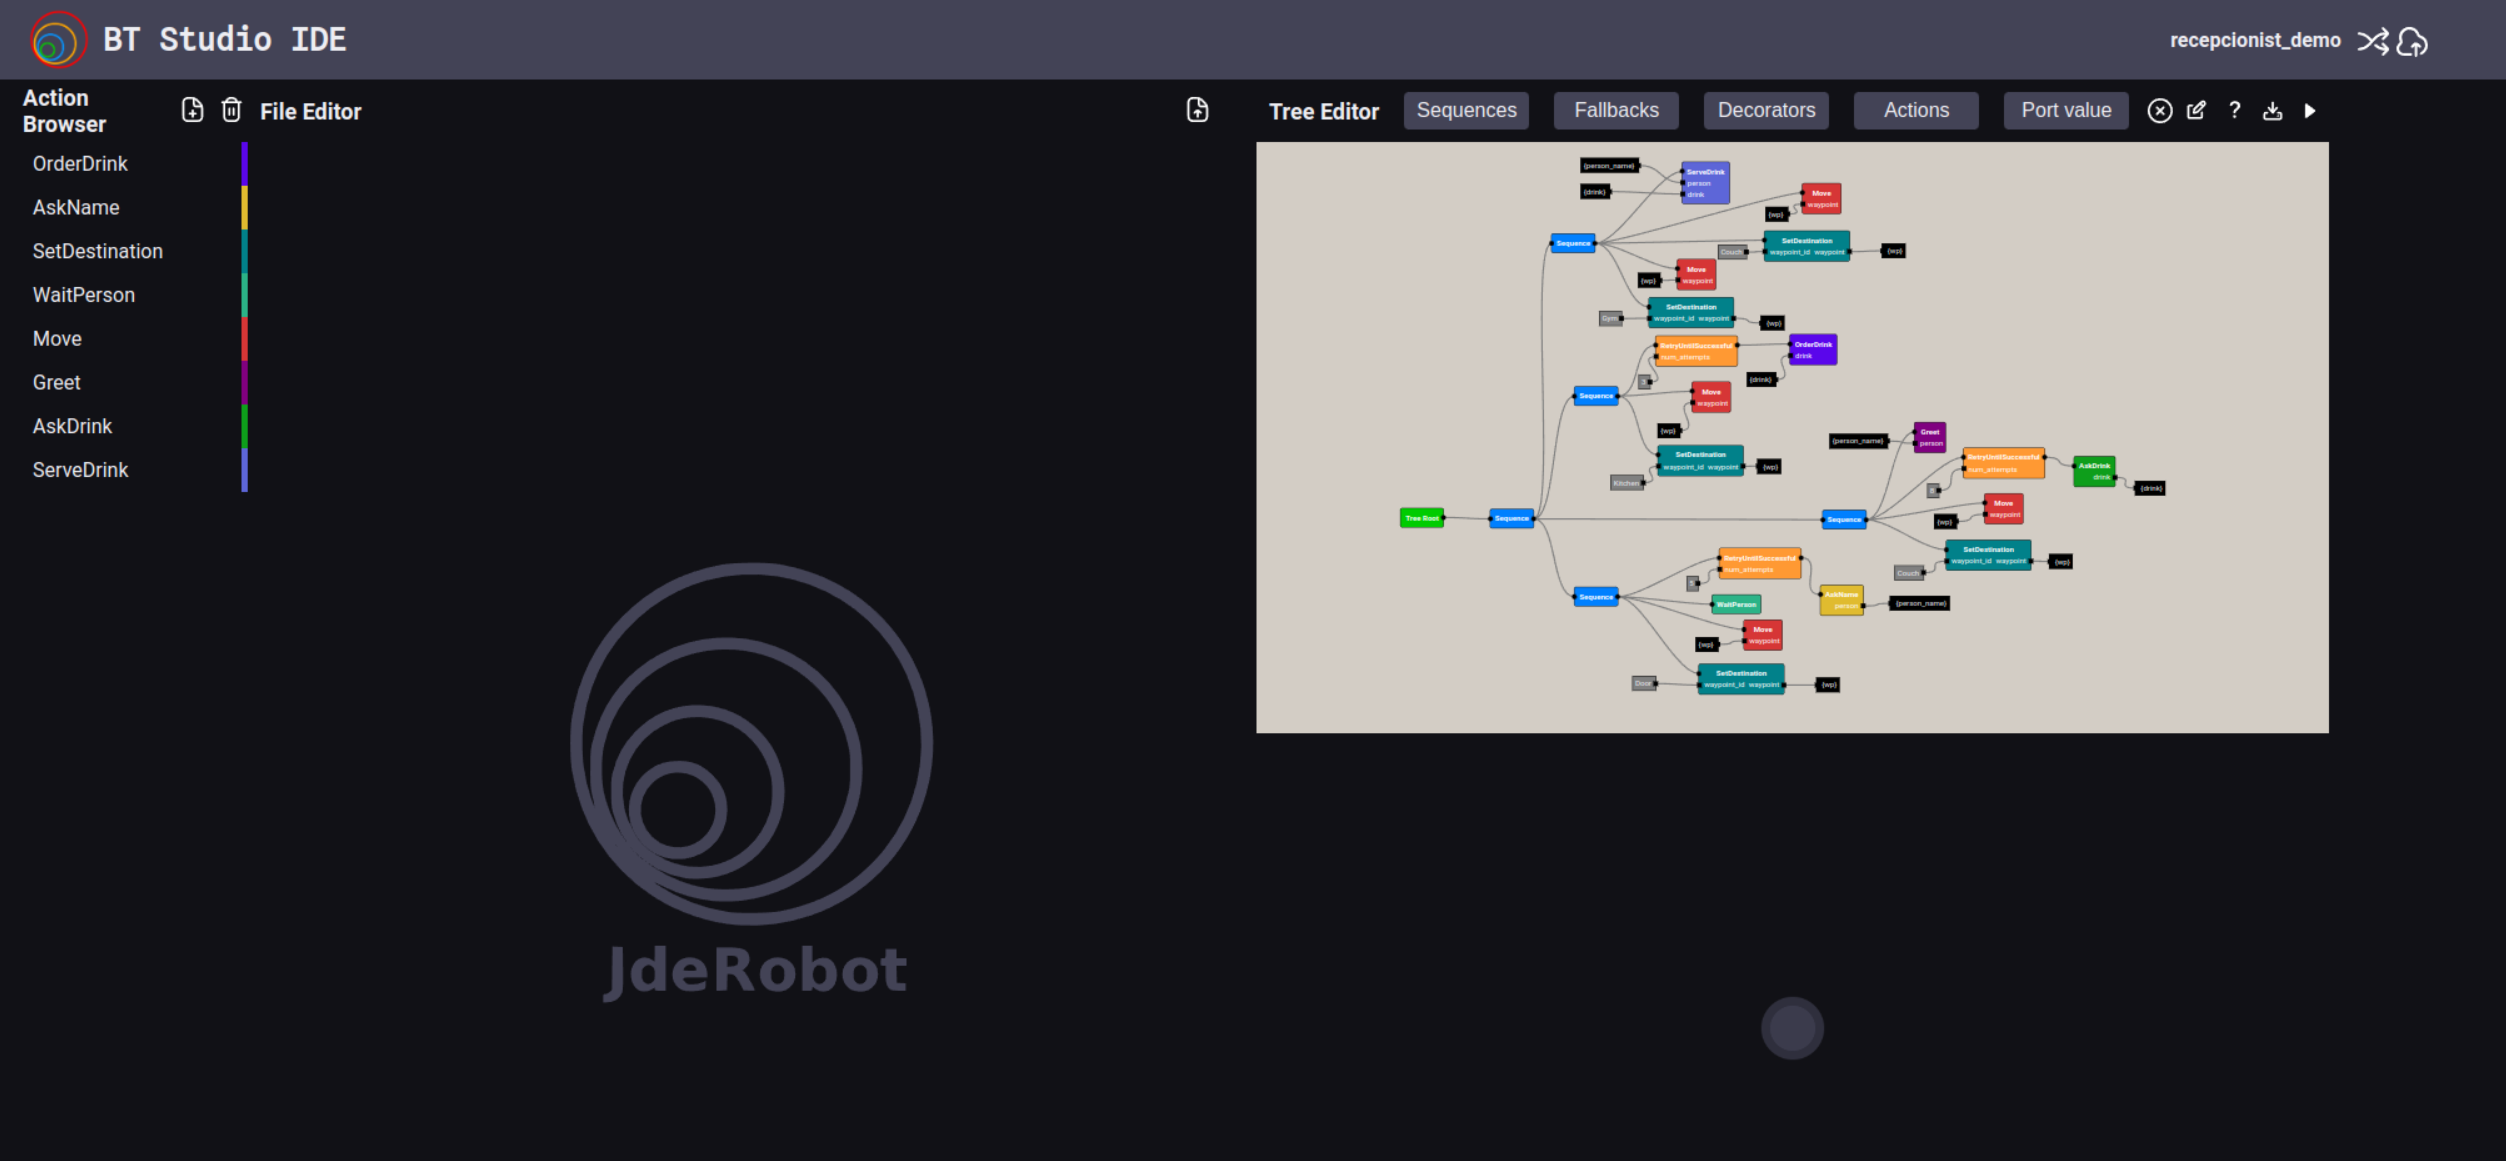
\includegraphics[width=6.6cm]{figs/screenshot1.png}}
  \end{figure}
  
\newpage
\slsubsect{User Interface}
\begin{itemize}
  \item \textbf{\textit{Text Editor}} + \textbf{\textit{{BT Editor}}} + \textbf{\textit{Vnc Visualizer}}
  \item Program the actions while modifying the behaviour tree \normalsize

\end{itemize}
%\begin{center}
  \begin{figure}
    \hspace{1cm}
    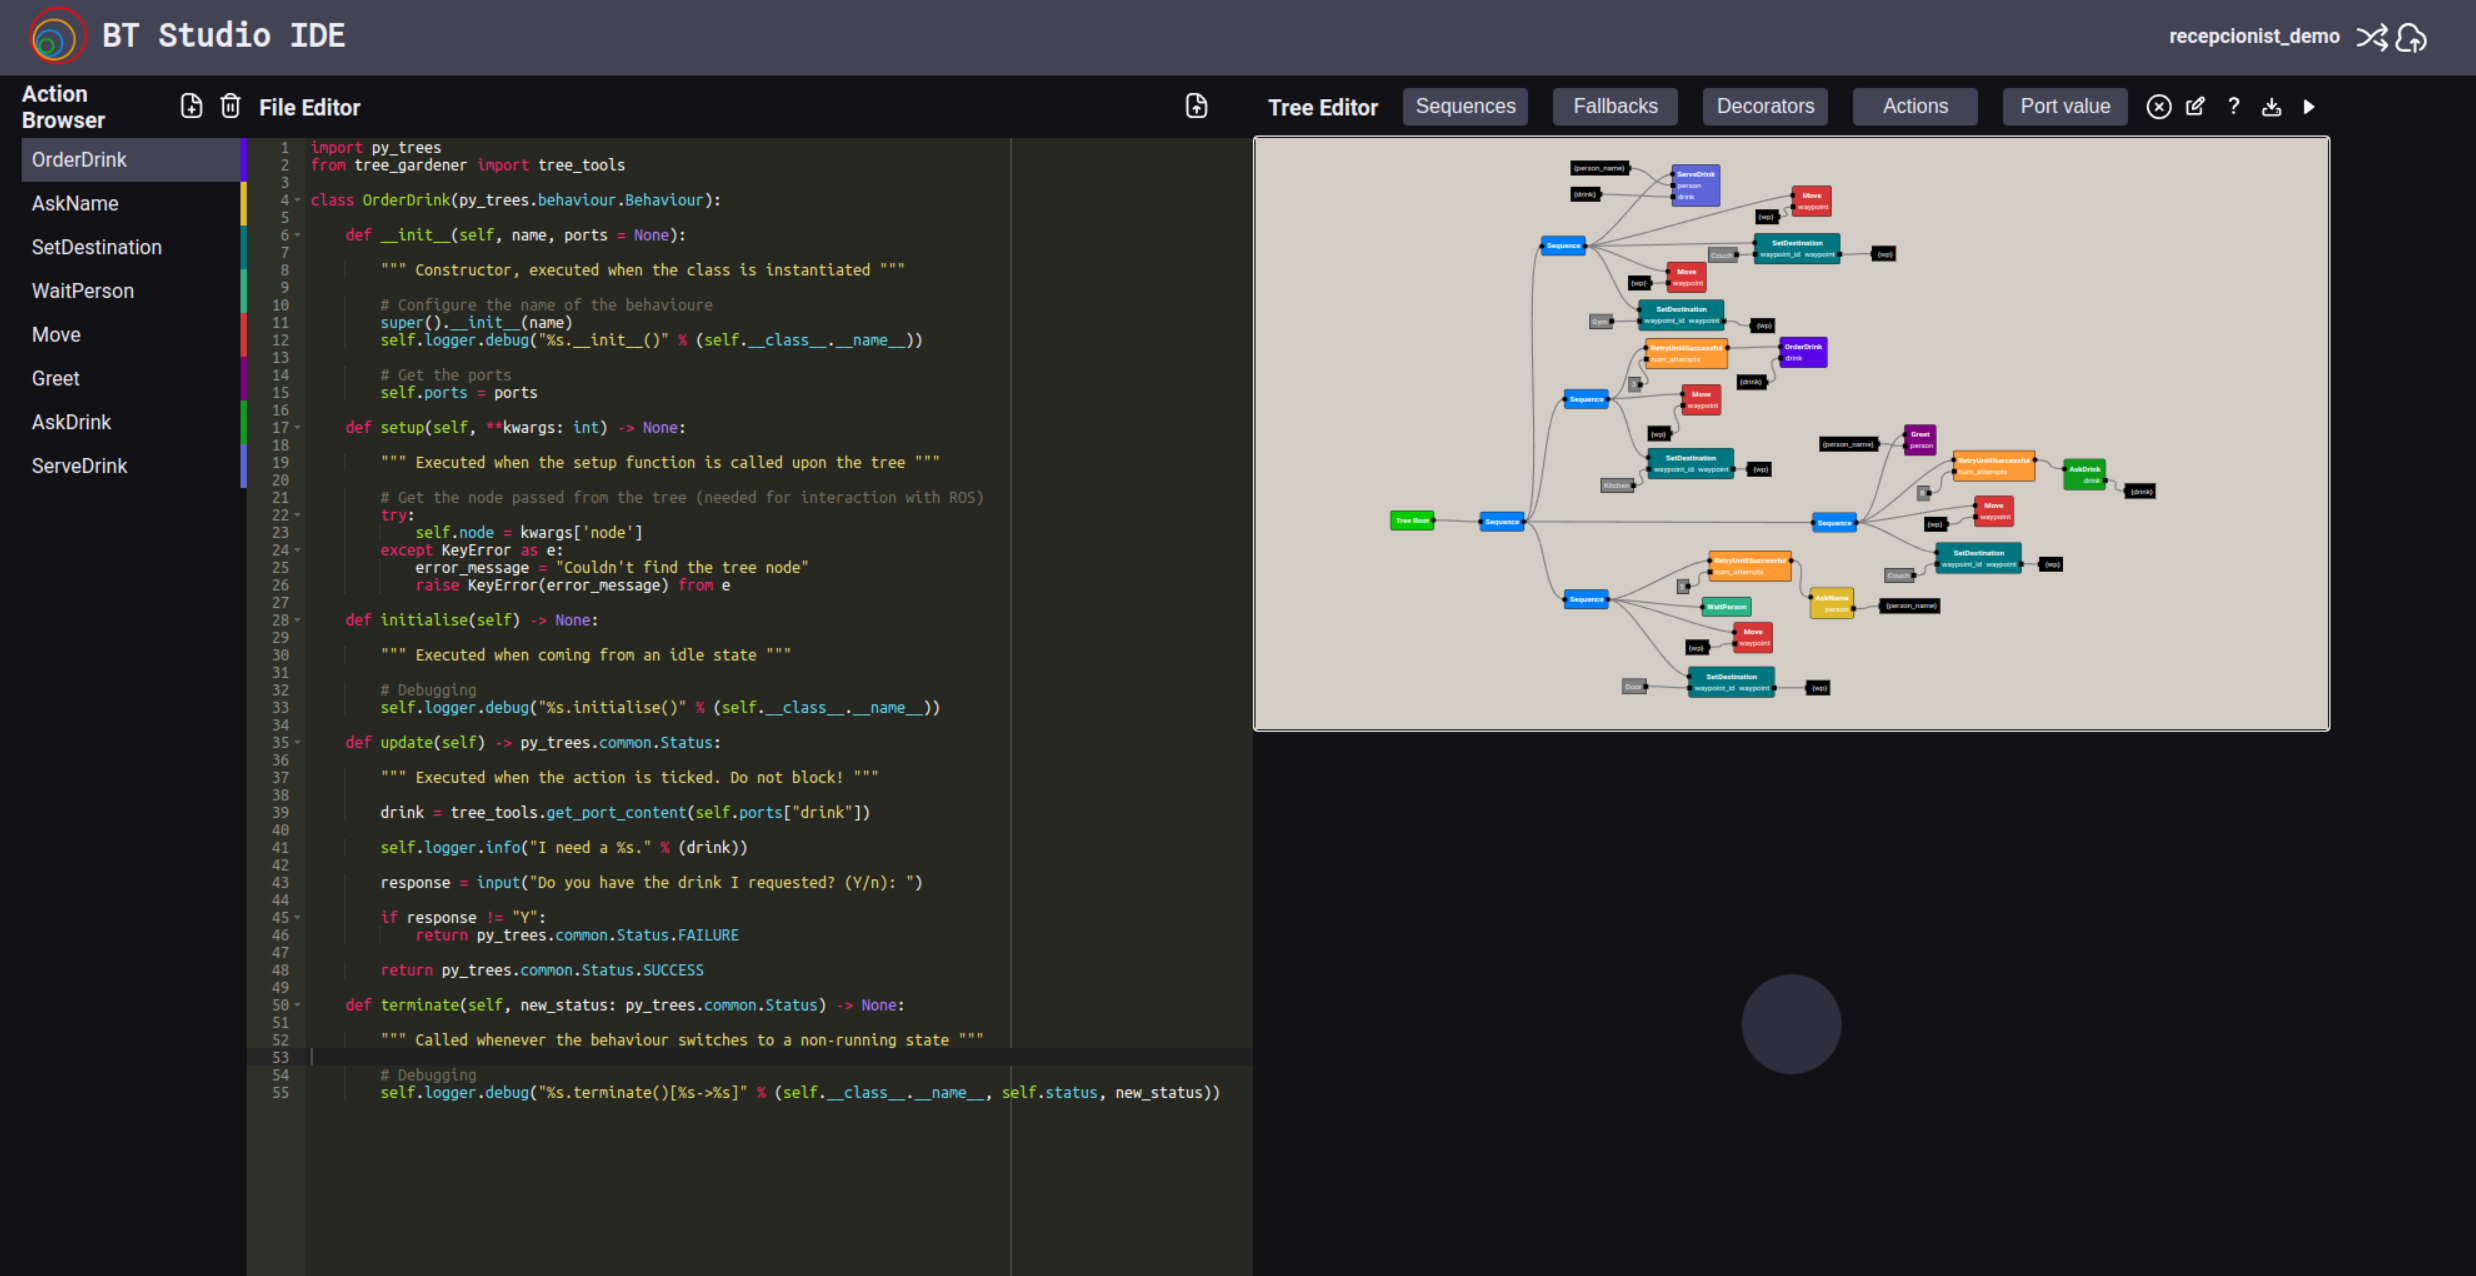
\includegraphics[width=9.5cm]{figs/screenshot3.png}
\end{figure}
%\end{center}

\newpage
\slsubsect{Behavior Tree Editor}
\begin{minipage}[t]{6.5cm}
  \vspace{0.5cm}
\begin{itemize}
\item Intuitive and reactive editor
\item Customizable colors for each action
\item Order from bottom to top
\item Everything you need for developing BT based applications
%\item Torneos
\end{itemize}
\end{minipage}
%\begin{minipage}[t]{4.5cm}
\begin{minipage}[t]{4.5cm}
	%\vspace{2.8cm}
	\begin{figure}
		\hspace{0.5cm}
		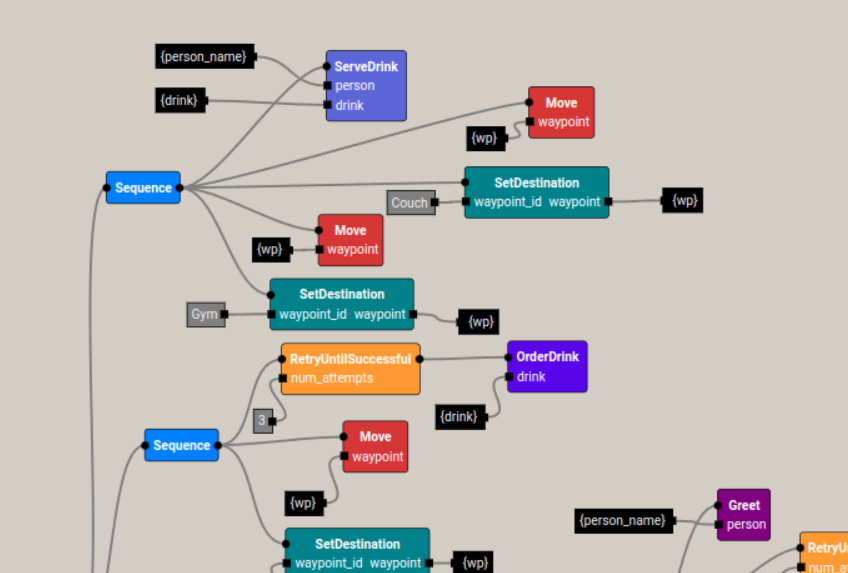
\includegraphics[width=4.6cm]{figs/screenshot2.png}
	\end{figure}
\end{minipage}
%\end{minipage}

\end{hslide}

\begin{hslide}
\slsect{Developers: How it works?}
\begin{minipage}[t]{7cm}
    \begin{itemize}
    \item Web tecnologies
      \begin{itemize}
      \item backend: Django
      \item frontend: React, HTML5, CSS
        %websockets
      \end{itemize}
    \item Robotics tecnologies
      \begin{itemize}
      \item ROS2
      \item Based around py\_trees
      \end{itemize}
    \item DevOps tecnologies
      \begin{itemize}
      \item Docker
      \end{itemize}
    \end{itemize}
\end{minipage}
\begin{minipage}[t]{5cm}
  \begin{figure}
    \centerline{
\includegraphics[width=4cm]{figs/html5.png}}
    
\includegraphics[width=1.5cm]{figs/Django-Logo.png}
    
\includegraphics[width=2cm]{figs/react-logo.png}
    
\includegraphics[width=1.6cm]{figs/docker-logo.png}\\
    
\includegraphics[width=1.5cm]{figs/Ros-logo.png}
  \end{figure}
\end{minipage}


\newpage
  \slsubsect{Action Structure}
  \begin{itemize}
  \item The structure is the same as py\_trees actions
  \end{itemize}
 \begin{figure}
    \centerline{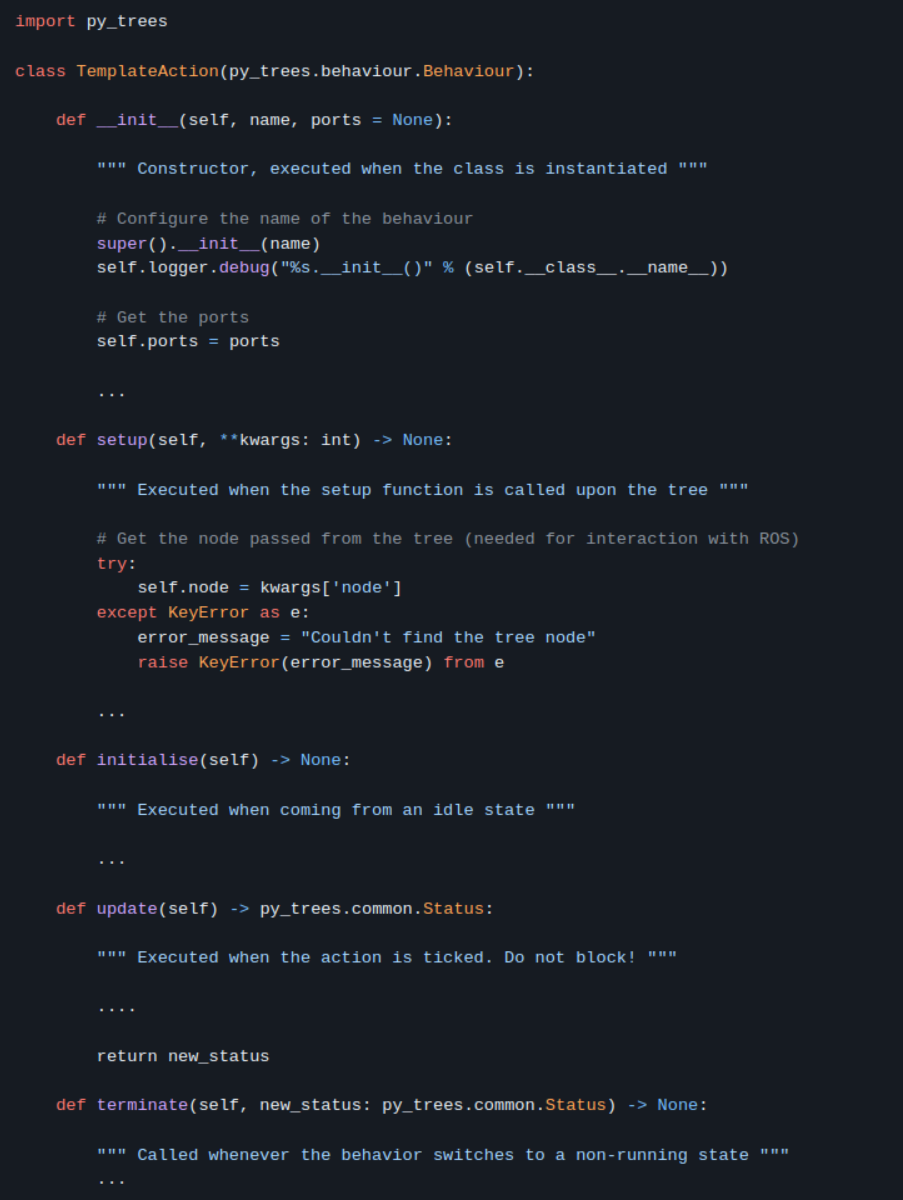
\includegraphics[height=6cm]{figs/screenshot4.png}}
 \end{figure}
 
\newpage
 \slsubsect{Traslation process}
 \begin{itemize}
 	\item Traslating from the user code and the diagram is done in the backend
 	\item The 2 parts are combined into a xml single file divided into 2 sections: the BaheviorTree and the Code
 	\item In the BehaviorTree section resides the Behavior Tree and is the same as what is generated by Groot2.
 	\item The code section is used instead of external files for containing each action source code
 \end{itemize}
 
 \newpage
 \slsubsect{Application Package}
 \begin{itemize}
 \item ROS2 humble is needed
 \item A testing enviroment is provided with the Webots simulator and a tree execution visualizer as thirdparty repos.
 \item Compile and run the app using the executor provided
 \item The actions and behaviour tree are merged into a single xml source file.
% \item 1 manager, \textit{n} ejercicios
 \end{itemize}

 \newpage
  \begin{minipage}[t]{7cm}
	\vspace{2cm}
  	\begin{itemize}
	  	\item \texttt{app\_tree.xml}: behavior tree and source code
		\item \texttt{execute.py}: launcher for the application
		\item \texttt{execute\_docker.py}: launcher for dockerized execution
		\item The rest is the same as a basic ROS package
	\end{itemize}
  \end{minipage}
  \begin{minipage}[t]{5cm}
  	\begin{figure}
  		\centerline{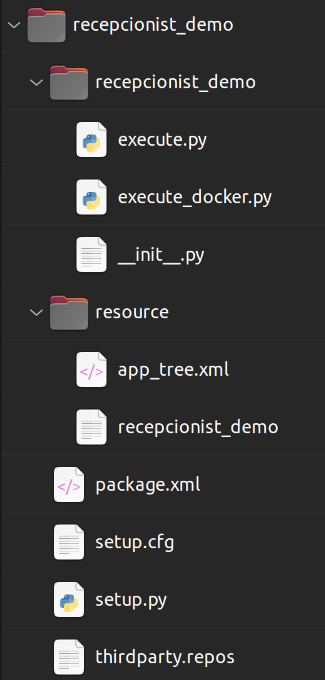
\includegraphics[height=7.2cm]{figs/package-struct.png}}
  	\end{figure}
  \end{minipage}
 
 \newpage
 \slsubsect{Dockerized execution}
 \begin{itemize}
 	\item Wait first to get it working
 	\item Using the Robotics Backend docker for easy development and ready to use templates.
\end{itemize} 
\end{hslide}

\begin{hslide}
  \slsect{For the future}
  \begin{itemize}
  \item Merge in Unibotics, online execution.
  \item Configure launchers
  \end{itemize}
\end{hslide}

\begin{hslide}
	\slsect{Working demos}
	\slsubsect{Recepcionist Demo}
	\begin{minipage}[t]{6.5cm}
		%  \vspace{0.5cm}
		\begin{itemize}
			\item Wait for dockerized execution
			%\item Autolocalización de robots
			% \item control visual
		\end{itemize}
		%\begin{figure}
		%  \hspace{1.5cm}
		%  \includegraphics[width=4cm]{figs/formula1-followline.png}
		%\end{figure}
		%\end{minipage}
		%\begin{minipage}[t]{4.5cm}
		%  \begin{figure}
			%    \includegraphics[width=3.5cm]{figs/vacuumcleaner.png}
			%    \includegraphics[width=3.5cm]{figs/laser-mapping.png}
			%  \end{figure}
	\end{minipage}
	
\end{hslide}

\end{document}

